% LaTex Template

\documentclass[12pt]{article}
%\usepackage{natbib}
\usepackage[letterpaper, margin=1.1in]{geometry}
\usepackage{graphicx}
\usepackage{wrapfig}
\usepackage{enumitem}
\setlist[enumerate]{itemsep=0mm}
\usepackage{multirow}
\usepackage[table,xcdraw]{xcolor}
\usepackage{lscape}
\usepackage{caption}
\usepackage{subcaption}
\usepackage{hyperref}

\begin{document}
\noindent{Alexandra Pulwicki \\ \today}

\begin{center}
\Large \textbf{Results\\ Point Scale}
\end{center}


\tableofcontents
\pagebreak

\section{Data normality}

A $\chi^2$ test was done to test whether the collected was normally distributed. The results are shown in Table \ref{tab:normality}. Generally, the data is not normally distributed and is strongly not normal when considering data from an entire glacier.

\begin{wraptable}{L}{8cm}
\centering
\caption{Normality of data with various subgroups. $\chi^2$ values are shown and normally distributed data is bold ($\alpha=0.10$ and $p<0.05$).}
\label{tab:normality}
\begin{tabular}{cccc}
\textbf{Glacier} & \textbf{Pattern} & \multicolumn{2}{c}{\textbf{$\chi^2$}} \\ 
\hline
\hline
\rowcolor[HTML]{EFEFEF} 
\cellcolor[HTML]{EFEFEF} & LH & 14.9 & \cellcolor[HTML]{EFEFEF} \\
\rowcolor[HTML]{EFEFEF} 
\cellcolor[HTML]{EFEFEF} & LC & 17.3 & \cellcolor[HTML]{EFEFEF} \\
\rowcolor[HTML]{EFEFEF} 
\cellcolor[HTML]{EFEFEF} & LM & 6.6 & \cellcolor[HTML]{EFEFEF} \\
\rowcolor[HTML]{EFEFEF} 
\cellcolor[HTML]{EFEFEF} & UH & 52.1 & \cellcolor[HTML]{EFEFEF} \\
\rowcolor[HTML]{EFEFEF} 
\cellcolor[HTML]{EFEFEF} & UC & \textbf{5.9} & \cellcolor[HTML]{EFEFEF} \\
\rowcolor[HTML]{EFEFEF} 
\cellcolor[HTML]{EFEFEF} & UM & \textbf{1.4} & \cellcolor[HTML]{EFEFEF} \\
\rowcolor[HTML]{EFEFEF} 
\multirow{-7}{*}{\cellcolor[HTML]{EFEFEF}G04} & UT & 15.7 & \multirow{-7}{*}{\cellcolor[HTML]{EFEFEF}115.4} \\
 & LH & 27.8 &  \\
 & LC & \textbf{5.0} &  \\
 & LM & \textbf{6.2} &  \\
 & UH & 43.8 &  \\
 & UC & 13.1 &  \\
 & UM & 31.3 &  \\
 & UT & \textbf{0.1} &  \\
\multirow{-8}{*}{G02} & BT & 13.1 & \multirow{-8}{*}{127.1} \\
\rowcolor[HTML]{EFEFEF} 
\cellcolor[HTML]{EFEFEF} & LH & 32.1 & \cellcolor[HTML]{EFEFEF} \\
\rowcolor[HTML]{EFEFEF} 
\cellcolor[HTML]{EFEFEF} & LC & 11.4 & \cellcolor[HTML]{EFEFEF} \\
\rowcolor[HTML]{EFEFEF} 
\cellcolor[HTML]{EFEFEF} & LM & 18.1 & \cellcolor[HTML]{EFEFEF} \\
\rowcolor[HTML]{EFEFEF} 
\cellcolor[HTML]{EFEFEF} & UH & 12.8 & \cellcolor[HTML]{EFEFEF} \\
\rowcolor[HTML]{EFEFEF} 
\cellcolor[HTML]{EFEFEF} & UC & 17.6 & \cellcolor[HTML]{EFEFEF} \\
\rowcolor[HTML]{EFEFEF} 
\cellcolor[HTML]{EFEFEF} & UM & 9.7 & \cellcolor[HTML]{EFEFEF} \\
\rowcolor[HTML]{EFEFEF} 
\multirow{-7}{*}{\cellcolor[HTML]{EFEFEF}G13} & UT & 8.6 & \multirow{-7}{*}{\cellcolor[HTML]{EFEFEF}39.4}
\end{tabular}
\end{wraptable}


\section{Observer differences}

A one-way ANOVA for each transect pattern of snow depth measurements taken by different observers  shows that there are no differences between observers. The only exception is the Lower Hourglass on Glacier 4, where one observer had higher mean snow depth than the other two (p $<$ 0.05). Since this was the first transect completed and the only one to show difference in observer measurements, there is cause to consider this an anomaly. This result shows that observer bias is not present in this study and no corrections to the data based on observer were applied.

\section{Standard deviation of snow depth along linear and curvilinear transects}

The \textit{mean} standard deviation of snow depth measurements taken at each location within various groups can be seen in Table \ref{tab:std_reproduce}. This value was found by calculating the standard deviation of three to four measurement done by each person at each measurement location. The mean of these standard deviations for each grouping, as show in Table \ref{tab:std_reproduce} and as a percent of the group mean in Table \ref{tab:std_reproduce_percent}, represents the variability in snow depth for the sampling locations. It can be used to evaluate the representativeness of the mean snow depth values that were used in analysis at larger scales.

The \textit{overall} standard deviation of all measurements within a certain grouping is shown in Table \ref{tab:std_measure} and as a percent of the group mean in Table \ref{tab:std_measure_percent}. These values were calculated by taking all the depth measurements within the groups defined in the table and then calculating the standard deviation. These values represent the variability in the depth field. 

The \textit{mean} standard deviation varies between glaciers, patterns, and observers but overall, the reproducibility of depth measurement is on the order of centimetres. This is a small variability compared to the \textit{overall} standard deviation of measurements. The standard deviation of measurements over the study area is on the order of 10$^1$, while the standard deviation of measurement reproducibility is on the order of 10$^0$. When expressed as a percentage of the mean, the \textit{overall} standard deviation for groups (Table \ref{tab:std_measure_percent}) is generally quite large and definitely larger than that of the \textit{mean} standard deviation (Table \ref{tab:std_reproduce_percent}). This shows that variability at the point scale (a single measurement) is an order of magnitude larger than the variability of the study area, so the use of the mean snow depth at each measurement location is a valid value to carry forward in the analysis. 

Variability in snow depth differs considerably between glaciers, as can be seen in Figure \ref{fig:box_depth}. Both the range and mean depth are largest for Glacier 4 and smallest for Glacier 13. Glacier 13 has the most outliers (\textgreater 1.5 $\times$ inner quartile range), which could be a result of a prominent surface meltwater channel. Overall glacier standard deviation (Table \ref{tab:std_measure}) is lowest for Glacier 13 and highest for Glacier 2, which the standard deviation of Glacier 4 being close to that of Glacier 2. 

The standard deviation as a function of binned elevation is shown in Figure \ref{fig:std_binned} as an absolute value and in Figure \ref{fig:std_binned_percent} as a percent of the mean. Both figures show that the standard deviation decreases with elevation on both Glacier 2 and 13 but it increases with elevation on Glacier 4, although this second relationship is quite weak. Therefore, the variability is higher closer to the terminus of the glacier. This result is likely skewed however because of the comparatively fewer depth measurements taken at higher elevations. 

%% Std of reproducibility
\begin{table}[]
\centering
\caption{\textit{Mean} standard deviation (cm) of snow depth measurements for various groupings.}
\label{tab:std_reproduce}
\begin{tabular}{cccccccc}
 &  &  &  & \multicolumn{4}{c}{\textbf{Person}} \\
\multirow{-2}{*}{\textbf{Glacier}} & \multirow{-2}{*}{\textbf{Pattern}} & \multirow{-2}{*}{\textbf{\begin{tabular}[c]{@{}c@{}}Overall \\ Glacier\end{tabular}}} & \multirow{-2}{*}{\textbf{\begin{tabular}[c]{@{}c@{}}Overall \\ Pattern\end{tabular}}} & AP & GF & CA & AC \\ \hline
\rowcolor[HTML]{EFEFEF} 
\cellcolor[HTML]{EFEFEF} & LH & \cellcolor[HTML]{EFEFEF} & 5.1 & 4.8 & --- & 8.5 & 2 \\
\rowcolor[HTML]{EFEFEF} 
\cellcolor[HTML]{EFEFEF} & LC & \cellcolor[HTML]{EFEFEF} & 4.7 & 4.3 & --- & 8.2 & 1.7 \\
\rowcolor[HTML]{EFEFEF} 
\cellcolor[HTML]{EFEFEF} & LM & \cellcolor[HTML]{EFEFEF} & 3.7 & --- & 4.7 & 4.6 & 1.9 \\
\rowcolor[HTML]{EFEFEF} 
\cellcolor[HTML]{EFEFEF} & UH & \cellcolor[HTML]{EFEFEF} & 2.6 & 3.4 & 2.2 & --- & 2.3 \\
\rowcolor[HTML]{EFEFEF} 
\cellcolor[HTML]{EFEFEF} & UC & \cellcolor[HTML]{EFEFEF} & 1.9 & 1.9 & 2.3 & --- & 1.5 \\
\rowcolor[HTML]{EFEFEF} 
\cellcolor[HTML]{EFEFEF} & UM & \cellcolor[HTML]{EFEFEF} & 1.9 & --- & 1.7 & 2 & 2 \\
\rowcolor[HTML]{EFEFEF} 
\multirow{-7}{*}{\cellcolor[HTML]{EFEFEF}Glacier 4} & UT & \multirow{-7}{*}{\cellcolor[HTML]{EFEFEF}3.5} & 3.9 & 3.7 & --- & 2.4 & 5.6 \\
 & LH &  & 5.4 & 4.8 & --- & 6.1 & --- \\
 & LC &  & 5 & 3.9 & --- & 6.2 & --- \\
 & LM &  & 6.5 & --- & 6.8 & 6.5 & 6 \\
 & UH &  & 4.1 & 3.5 & 4.4 & 4.5 & --- \\
 & UC &  & 7 & 5.5 & 7 & 8.7 & --- \\
 & UM &  & 4.2 & 3.2 & 5.2 & 4.1 & --- \\
 & UT &  & 5.6 & 3.2 & --- & 8.2 & --- \\
\multirow{-8}{*}{Glacier 2} & BT & \multirow{-8}{*}{5.1} & 2.2 & 2.2 & --- & 3 & 1.5 \\
\rowcolor[HTML]{EFEFEF} 
\cellcolor[HTML]{EFEFEF} & LH & \cellcolor[HTML]{EFEFEF} & 3.8 & 3.1 & 4.1 & 4 & --- \\
\rowcolor[HTML]{EFEFEF} 
\cellcolor[HTML]{EFEFEF} & LC & \cellcolor[HTML]{EFEFEF} & 4.5 & 2.9 & 4.8 & 5.8 & --- \\
\rowcolor[HTML]{EFEFEF} 
\cellcolor[HTML]{EFEFEF} & LM & \cellcolor[HTML]{EFEFEF} & 6.6 & 4.6 & 7.7 & 7.6 & --- \\
\rowcolor[HTML]{EFEFEF} 
\cellcolor[HTML]{EFEFEF} & UH & \cellcolor[HTML]{EFEFEF} & 3.5 & 3.4 & 3.6 & 3.4 & --- \\
\rowcolor[HTML]{EFEFEF} 
\cellcolor[HTML]{EFEFEF} & UC & \cellcolor[HTML]{EFEFEF} & 3.8 & 3.4 & 4 & 4 & --- \\
\rowcolor[HTML]{EFEFEF} 
\cellcolor[HTML]{EFEFEF} & UM & \cellcolor[HTML]{EFEFEF} & 4.8 & 4.4 & 5.8 & 4.4 & --- \\
\rowcolor[HTML]{EFEFEF} 
\multirow{-7}{*}{\cellcolor[HTML]{EFEFEF}Glacier 13} & UT & \multirow{-7}{*}{\cellcolor[HTML]{EFEFEF}4.2} & 4.1 & 2.7 & 4.8 & 4.6 & ---
\end{tabular}
\end{table}

%% Std of reproducibility
\begin{table}[]
\centering
\caption{\textit{Mean} standard deviation as percent of mean snow depth measurements for various groupings.}
\label{tab:std_reproduce_percent}
\begin{tabular}{cccccccc}
 &  &  &  & \multicolumn{4}{c}{\textbf{Person (\%)}} \\
\multirow{-2}{*}{\textbf{Glacier}} & \multirow{-2}{*}{\textbf{Pattern}} & \multirow{-2}{*}{\textbf{\begin{tabular}[c]{@{}c@{}}Overall \\ Glacier (\%)\end{tabular}}} & \multirow{-2}{*}{\textbf{\begin{tabular}[c]{@{}c@{}}Overall \\ Pattern (\%)\end{tabular}}} & AP & GF & CA & AC \\ \hline
\rowcolor[HTML]{EFEFEF} 
\cellcolor[HTML]{EFEFEF} & LH & \cellcolor[HTML]{EFEFEF} & 3 & 3 & --- & 5 & 1 \\
\rowcolor[HTML]{EFEFEF} 
\cellcolor[HTML]{EFEFEF} & LC & \cellcolor[HTML]{EFEFEF}  & 3 & 3 & --- & 5 & 1 \\
\rowcolor[HTML]{EFEFEF} 
\cellcolor[HTML]{EFEFEF} & LM & \cellcolor[HTML]{EFEFEF} & 2 & --- & 3 & 2 & 1 \\
\rowcolor[HTML]{EFEFEF} 
\cellcolor[HTML]{EFEFEF} & UH & \cellcolor[HTML]{EFEFEF} &1 & 1 & 1 & --- &1 \\
\rowcolor[HTML]{EFEFEF} 
\cellcolor[HTML]{EFEFEF} & UC & \cellcolor[HTML]{EFEFEF} &1 & 2 & 1 & --- &1 \\
\rowcolor[HTML]{EFEFEF} 
\cellcolor[HTML]{EFEFEF} & UM & \cellcolor[HTML]{EFEFEF} & 1& --- & 1 & 1 & 1 \\
\rowcolor[HTML]{EFEFEF} 
\multirow{-7}{*}{\cellcolor[HTML]{EFEFEF}Glacier 4} & UT & \multirow{-7}{*}{\cellcolor[HTML]{EFEFEF}2} & 2& 2 & --- & 1 & 3 \\
 & LH &  & 11 & 9 & --- & 13 & --- \\
 & LC &  & 12 & 11 & --- & 15 & --- \\
 & LM &  & 17 & --- &16  & 18 & 16 \\
 & UH &  & 7 & 5 & 7 & 9 & --- \\
 & UC &  & 4 & 3& 4 & 4 & --- \\
 & UM &   & 4 & 3& 4 & 4  & --- \\
 & UT &  & 10 & 6 & --- & 13 & --- \\
\multirow{-8}{*}{Glacier 2} & BT & \multirow{-8}{*}{7} &2 &2 & --- & 2 & 1 \\
\rowcolor[HTML]{EFEFEF} 
\cellcolor[HTML]{EFEFEF} & LH & \cellcolor[HTML]{EFEFEF} & 10 & 6 & 12 & 13 & --- \\
\rowcolor[HTML]{EFEFEF} 
\cellcolor[HTML]{EFEFEF} & LC & \cellcolor[HTML]{EFEFEF} & 8 & 6 & 9 & 8 & --- \\
\rowcolor[HTML]{EFEFEF} 
\cellcolor[HTML]{EFEFEF} & LM & \cellcolor[HTML]{EFEFEF} & 13 & 10 & 16 & 14 & --- \\
\rowcolor[HTML]{EFEFEF} 
\cellcolor[HTML]{EFEFEF} & UH & \cellcolor[HTML]{EFEFEF} & 4 & 4 & 5 & 5 & --- \\
\rowcolor[HTML]{EFEFEF} 
\cellcolor[HTML]{EFEFEF} & UC & \cellcolor[HTML]{EFEFEF} & 4 & 4 &  4 & 4 & --- \\
\rowcolor[HTML]{EFEFEF} 
\cellcolor[HTML]{EFEFEF} & UM & \cellcolor[HTML]{EFEFEF} &6 & 5 & 7 & 5 & --- \\
\rowcolor[HTML]{EFEFEF} 
\multirow{-7}{*}{\cellcolor[HTML]{EFEFEF}Glacier 13} & UT & \multirow{-7}{*}{\cellcolor[HTML]{EFEFEF}6} & 6 & 4 & 6 & 7 & ---
\end{tabular}
\end{table}

%% Std of measurement
\begin{table}[]
\centering
\caption{\textit{Overall} standard deviation (cm) of snow depth measurements for various groupings. The standard deviation of all transect data was 64.6 cm.}
\label{tab:std_measure}
\begin{tabular}{cccccccc}
 &  &  &  & \multicolumn{4}{l}{\textbf{Person}} \\
\multirow{-2}{*}{\textbf{Glacier}} & \multirow{-2}{*}{\textbf{Pattern}} & \multirow{-2}{*}{\textbf{\begin{tabular}[c]{@{}l@{}}Overall \\ Glacier\end{tabular}}} & \multirow{-2}{*}{\textbf{\begin{tabular}[c]{@{}l@{}}Overall \\ Pattern\end{tabular}}} & AP & GF & CA & AC \\ \hline
\rowcolor[HTML]{EFEFEF} 
\cellcolor[HTML]{EFEFEF} & LH & \cellcolor[HTML]{EFEFEF} & 51.3 & 51.4 & --- & 54.8 & 45.7 \\
\rowcolor[HTML]{EFEFEF} 
\cellcolor[HTML]{EFEFEF} & LC & \cellcolor[HTML]{EFEFEF} & 45.2 & 50.5 & --- & 44.1 & 39.8 \\
\rowcolor[HTML]{EFEFEF} 
\cellcolor[HTML]{EFEFEF} & LM & \cellcolor[HTML]{EFEFEF} & 27.2 & --- & 21.6 & 36.3 & 22.5 \\
\rowcolor[HTML]{EFEFEF} 
\cellcolor[HTML]{EFEFEF} & UH & \cellcolor[HTML]{EFEFEF} & 48.5 & 48.6 & 51.2 & --- & 45.8 \\
\rowcolor[HTML]{EFEFEF} 
\cellcolor[HTML]{EFEFEF} & UC & \cellcolor[HTML]{EFEFEF} & 44.2 & 44.8 & 38.2 & --- & 48.2 \\
\rowcolor[HTML]{EFEFEF} 
\cellcolor[HTML]{EFEFEF} & UM & \cellcolor[HTML]{EFEFEF} & 22.5 & --- & 24.1 & 20.7 & 22.7 \\
\rowcolor[HTML]{EFEFEF} 
\multirow{-7}{*}{\cellcolor[HTML]{EFEFEF}Glacier 4} & UT & \multirow{-7}{*}{\cellcolor[HTML]{EFEFEF}44.7} & 26 & 25.1 & --- & 25.1 & 27.7 \\
 & LH &  & 29.9 & 29.2 & --- & 30.6 & --- \\
 & LC &  & 29.3 & 28.6 & --- & 30.1 & --- \\
 & LM &  & 18.4 & --- & 20.8 & 15.5 & 18.1 \\
 & UH &  & 42 & 39.1 & 41.6 & 45.6 & --- \\
 & UC &  & 55 & 55.3 & 55.2 & 56.1 & --- \\
 & UM &  & 35.1 & 38.4 & 34.5 & 31.8 & --- \\
 & UT &  & 36.4 & 27.3 & --- & 43.9 & --- \\
\multirow{-8}{*}{Glacier 2} & BT & \multirow{-8}{*}{49.3} & 20.8 & 13.8 & --- & 13.7 & 30.4 \\
\rowcolor[HTML]{EFEFEF} 
\cellcolor[HTML]{EFEFEF} & LH & \cellcolor[HTML]{EFEFEF} & 27.4 & 25.7 & 27.5 & 28.9 & --- \\
\rowcolor[HTML]{EFEFEF} 
\cellcolor[HTML]{EFEFEF} & LC & \cellcolor[HTML]{EFEFEF} & 27.1 & 25.8 & 21.4 & 32.6 & --- \\
\rowcolor[HTML]{EFEFEF} 
\cellcolor[HTML]{EFEFEF} & LM & \cellcolor[HTML]{EFEFEF} & 24.9 & 22.8 & 27.5 & 23.6 & --- \\
\rowcolor[HTML]{EFEFEF} 
\cellcolor[HTML]{EFEFEF} & UH & \cellcolor[HTML]{EFEFEF} & 21 & 21.1 & 21.4 & 20.4 & --- \\
\rowcolor[HTML]{EFEFEF} 
\cellcolor[HTML]{EFEFEF} & UC & \cellcolor[HTML]{EFEFEF} & 16.3 & 17.6 & 14.5 & 16.6 & --- \\
\rowcolor[HTML]{EFEFEF} 
\cellcolor[HTML]{EFEFEF} & UM & \cellcolor[HTML]{EFEFEF} & 29.4 & 26.6 & 33.4 & 28 & --- \\
\rowcolor[HTML]{EFEFEF} 
\multirow{-7}{*}{\cellcolor[HTML]{EFEFEF}Glacier 13} & UT & \multirow{-7}{*}{\cellcolor[HTML]{EFEFEF}30.5} & 32.7 & 21.5 & 44.4 & 26.4 & ---
\end{tabular}
\end{table}


%% Std of measurement
\begin{table}[]
\centering
\caption{\textit{Overall} standard deviation as percent of mean snow depth measurements for various groupings. The standard deviation as a percent of the mean of all transect data was 63\%.}
\label{tab:std_measure_percent}
\begin{tabular}{cccccccc}
 &  &  &  & \multicolumn{4}{l}{\textbf{Person (\%)}} \\
\multirow{-2}{*}{\textbf{Glacier}} & \multirow{-2}{*}{\textbf{Pattern}} & \multirow{-2}{*}{\textbf{\begin{tabular}[c]{@{}l@{}}Overall \\ Glacier (\%)\end{tabular}}} & \multirow{-2}{*}{\textbf{\begin{tabular}[c]{@{}l@{}}Overall \\ Pattern (\%)\end{tabular}}} & AP & GF & CA & AC \\ 
\hline
\hline
\rowcolor[HTML]{EFEFEF} 
\cellcolor[HTML]{EFEFEF} & LH & \cellcolor[HTML]{EFEFEF} & 28 & 29 & --- & 32 & 24 \\
\rowcolor[HTML]{EFEFEF} 
\cellcolor[HTML]{EFEFEF} & LC & \cellcolor[HTML]{EFEFEF} & 26 &30 & --- & 25 & 23 \\
\rowcolor[HTML]{EFEFEF} 
\cellcolor[HTML]{EFEFEF} & LM & \cellcolor[HTML]{EFEFEF} &15 & --- &11 & 19 & 12 \\
\rowcolor[HTML]{EFEFEF} 
\cellcolor[HTML]{EFEFEF} & UH & \cellcolor[HTML]{EFEFEF} & 28 & 28 & 29 & --- & 27 \\
\rowcolor[HTML]{EFEFEF} 
\cellcolor[HTML]{EFEFEF} & UC & \cellcolor[HTML]{EFEFEF} & 23 & 23 & 21 & --- & 26 \\
\rowcolor[HTML]{EFEFEF} 
\cellcolor[HTML]{EFEFEF} & UM & \cellcolor[HTML]{EFEFEF} & 13 & --- & 14 & 12 & 13 \\
\rowcolor[HTML]{EFEFEF} 
\multirow{-7}{*}{\cellcolor[HTML]{EFEFEF}Glacier 4} & UT & \multirow{-7}{*}{\cellcolor[HTML]{EFEFEF}25} & 13& 13 & --- & 13 & 14 \\
 & LH &  & 67 & 63 & --- & 71 & --- \\
 & LC &  & 61& 63 & --- & 59 & --- \\
 & LM &  &43& --- & 45 & 39& 43 \\
 & UH &  & 39 & 37 & 38 & 42 & --- \\
 & UC &  & 52 & 53 & 52 & 52 & --- \\
 & UM &  & 29 & 33 & 29 & 27 & --- \\
 & UT &  & 61 & 51 & --- & 70 & --- \\
\multirow{-8}{*}{Glacier 2} & BT & \multirow{-8}{*}{62} & 14 & 10 & --- & 9 & 22 \\
\rowcolor[HTML]{EFEFEF} 
\cellcolor[HTML]{EFEFEF} & LH & \cellcolor[HTML]{EFEFEF} & 56 & 53 & 58 & 57 & --- \\
\rowcolor[HTML]{EFEFEF} 
\cellcolor[HTML]{EFEFEF} & LC & \cellcolor[HTML]{EFEFEF} & 59 & 57 & 52 & 68 & --- \\
\rowcolor[HTML]{EFEFEF} 
\cellcolor[HTML]{EFEFEF} & LM & \cellcolor[HTML]{EFEFEF} & 52 & 60 &56 & 42 & --- \\
\rowcolor[HTML]{EFEFEF} 
\cellcolor[HTML]{EFEFEF} & UH & \cellcolor[HTML]{EFEFEF} &25 & 25 & 25 & 24 & --- \\
\rowcolor[HTML]{EFEFEF} 
\cellcolor[HTML]{EFEFEF} & UC & \cellcolor[HTML]{EFEFEF} & 18 & 21 & 16 & 18 & --- \\
\rowcolor[HTML]{EFEFEF} 
\cellcolor[HTML]{EFEFEF} & UM & \cellcolor[HTML]{EFEFEF} & 34 & 32 & 39 & 33 & --- \\
\rowcolor[HTML]{EFEFEF} 
\multirow{-7}{*}{\cellcolor[HTML]{EFEFEF}Glacier 13} & UT & \multirow{-7}{*}{\cellcolor[HTML]{EFEFEF}46} & 50 & 31 & 63 & 42 & ---
\end{tabular}
\end{table}



{
\begin{wrapfigure}{r}{\textwidth} 
\centering
	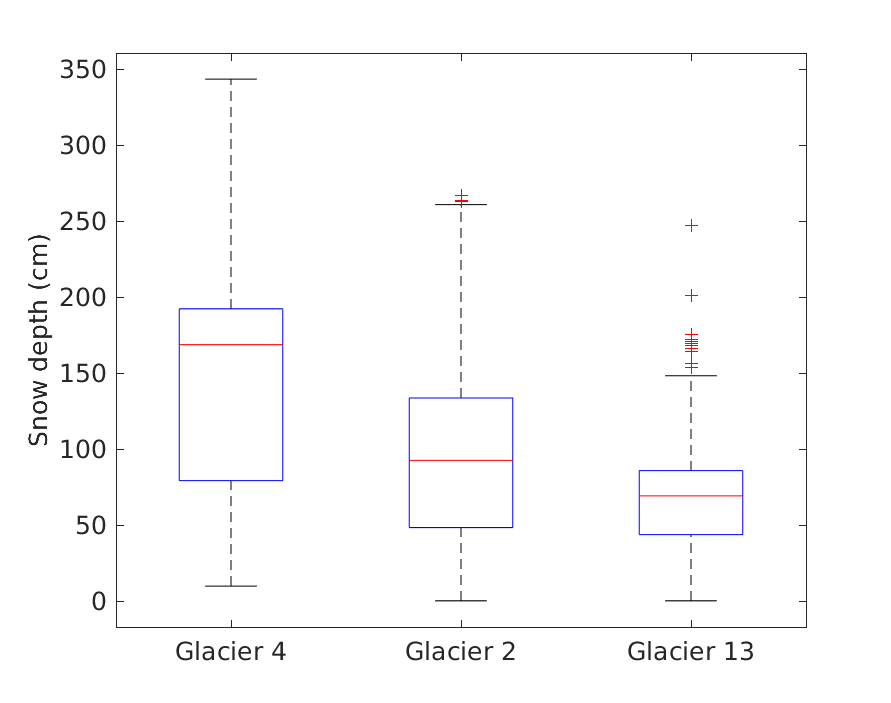
\includegraphics[height = 10cm]{box_depth.png}\\
	\caption{Variability in snow depth measurements taken at each glacier.}
	\label{fig:box_depth}
\end{wrapfigure}
}

{
\begin{wrapfigure}{r}{\textwidth} 
\centering
	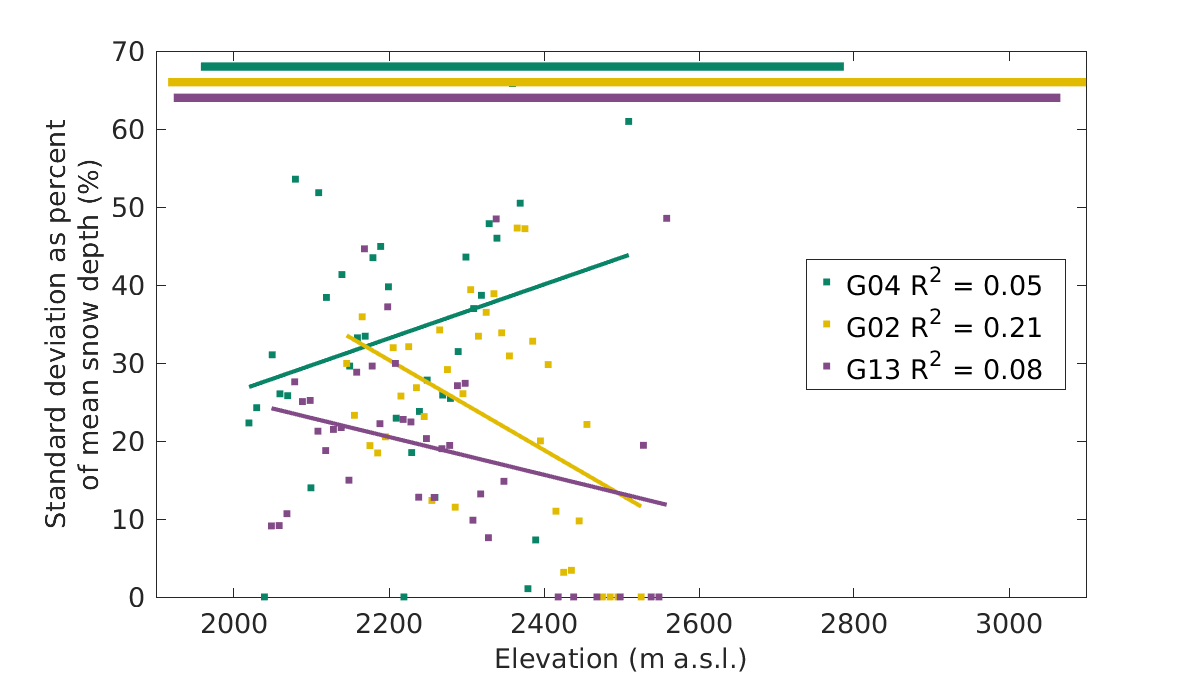
\includegraphics[height = 10cm]{binned_std.png}\\
	\caption{Standard deviation of all measurements binned in elevation bands of 10 m. Bars at the top of the figure indicate the elevation range of the three study glaciers.}
	\label{fig:std_binned}
\end{wrapfigure}
}

{
\begin{wrapfigure}{r}{\textwidth} 
\centering
	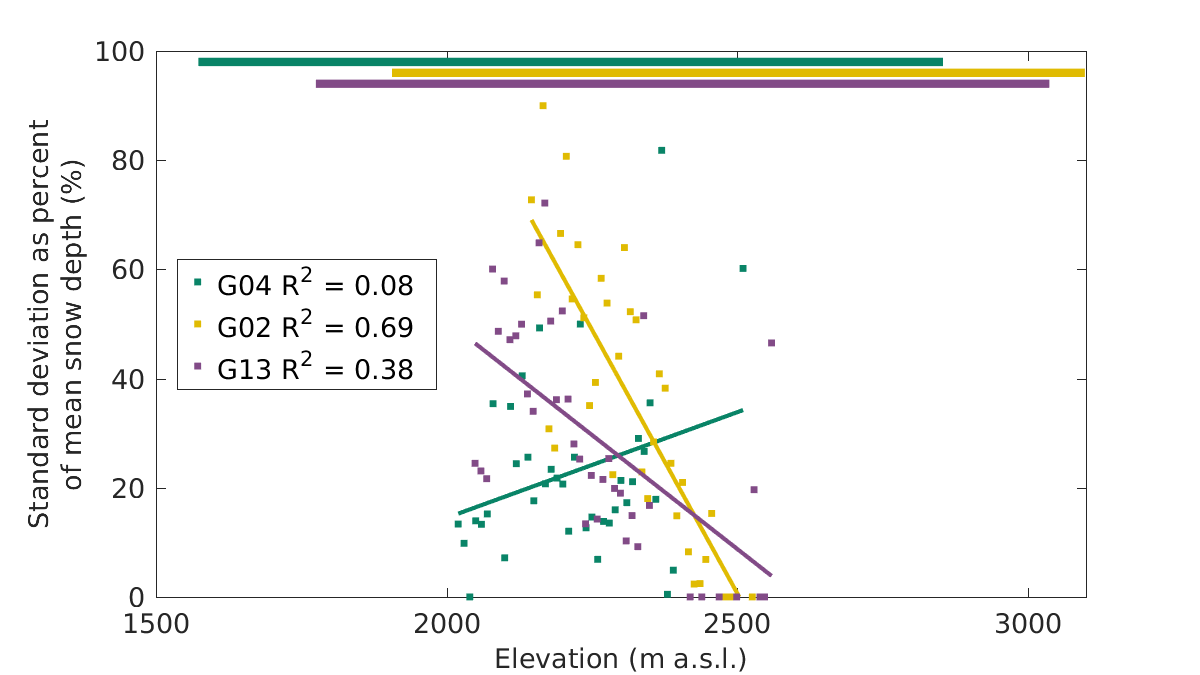
\includegraphics[height = 10cm]{binned_std_percent.png}\\
	\caption{Standard deviation as percent of mean measurements binned in elevation bands of 10 m. Bars at the top of the figure indicate the elevation range of the three study glaciers.}
	\label{fig:std_binned_percent}
\end{wrapfigure}
}













\end{document}
